\documentclass{article}
\usepackage[utf8]{inputenc}
\usepackage{hyperref}
\usepackage[left=20mm,top=20mm,right=20mm,bottom=20mm]{geometry}
\usepackage{etoolbox} %required for cover page
\usepackage{booktabs}
\usepackage[usestackEOL]{stackengine}
\usepackage[T1]{fontenc}
\usepackage[utf8]{inputenc}
\usepackage{bm}
\usepackage{graphicx}
\usepackage{subcaption}
\usepackage{amsmath}
\usepackage{amsfonts}
\usepackage{mathtools}
\usepackage{xcolor}
\usepackage{float}
\usepackage{hyperref}
\usepackage[capitalise]{cleveref}
\usepackage{enumitem,kantlipsum}
\usepackage{amssymb}
\usepackage[square,numbers,sort]{natbib}
\usepackage[ruled,vlined]{algorithm2e}
\usepackage{listings}
\usepackage{lscape}
\usepackage{longtable}
\usepackage{boldline}



\title{Laboratorio di Interazioni Fondamentali \\ Relazione esperienza 1}
\author{Irene Celestino}
\date{8/11/2022}

\begin{document}
\maketitle

\section{Introduzione e scopo dell'esperienza}
Lo scopo dell'esperienza preliminare è di usare per la prima volta i rivelatori di raggi cosmici, ovvero scintillatori e fotomoltiplicatori, e di stimare l'efficienza del secondo scintillatore posto più in alto. 
\\
\\
I vari step dell'esperienza sono: 
\begin{itemize}
    \item [1.] studio del segnale in uscita dai 3 fotomoltiplicatori al variare della tensione di alimentazione
    \item [2.] utilizzo delle unità di discriminazione e di coincidenza, analisi del segnale in uscita e stima del ritardo da loro introdotto 
    \item [3.] conteggio del numero di eventi registrati per unità di tempo dai singoli fotomoltiplicatori e in coincidenza doppia o tripla
    \item [4.] stima dell'efficienza del secondo scintillatore come $$\epsilon_2 = \frac{n(1\&2\&3)}{n(1\&3)}$$
\end{itemize}

\subsection{Apparato sperimentale}
Gli strumenti utilizzati sono: 
\begin{itemize}
    \item 3 scintillatori plastici 
    \item 3 fotomoltiplicatori (9954B dell'azienda ET Enterprises) posti più in alto (indicati nella relazione come PM7, PM5 e PM4) 
    \item 1 unità di discriminazione a 4 ingressi
    \item 2 unità di coincidenza a 5 ingressi ciascuna
    \item 1 contatore a 7 ingressi 
    \item il generatore di alta tensione e l'oscilloscopio digitale
\end{itemize}
L'apparato sperimentale è composto da 5 scintillatori plastici piani, di spessore di 2.5 cm e di forma data da un rettangolo di superficie 56 cm x 27 cm con poi una parte che va a stringersi sempre di più per arrivare al fotomoltiplicatore, lunga 30 cm.
posti uno sopra l'altro e ricoperti da un materiale di plastica nero che scherma l'apparato dalla luce ambientale. \\
La distanza tra il primo e il secondo è di 16 cm, mentre quella tra il secondo e il terzo è di 7 cm. 
A un'estremità di ogni scintillatore è collegato un fotomoltiplicatore, il cui segnale in uscita viene collegato al rack con un cavo coassiale nero di impedenza interna 50 Ohm e tempo di ritardo 6 ns.\\


\section{Studio del segnale del primo fotomoltiplicatore (PM7)}
\subsection{Visualizzazione del segnale all'oscilloscopio}
Per prima cosa, ho collegato i vari cavi a setup spento: 
\begin{itemize}
    \item il fotomoltiplicatore è collegato al rack con un cavo coassiale nero con impedenza interna 50 Ohm e tempo di ritardo 6 ns
    \item dal rack ho collegato il segnale in uscita da PM7 al CH1 dell'oscilloscopio, con un cavo coassiale con tempo di ritardo 2 ns e terminando la linea con una resistenza da 50 Ohm per evitare riflessioni
    \item ho impostato l'oscilloscopio digitale con le scale di 25.0 ns/div, 20 mV/div e con il trigger con sorgente CH1, slope falling, soglia -40 mV, mode Normal
\end{itemize}
Ho poi acceso l'alimentatore di tensione partendo da una tensione di alimentazione di 1100 V. Fino a 1600 V non si ha una frequenza di trigger superiore ai 10 Hz, mentre per le tensioni successive si hanno i seguenti risultati: 

\begin{center}
\begin{tabular}{|c|c|}
\hline
Tensione di alimentazione [kV] & Frequenza di trigger [Hz]\\
\hline
     1.600 & $<$ 10   \\
    1.700 & 10 $\div$ 30\\
    1.750  & 80 $\div$ 130\\
    1.770  & 120 $\div$ 200\\
    \hline
\end{tabular}
\end{center}
Il segnale è composto da un picco verso il basso, della durata media di 10 ns, con un paio di picchettini alti in media 4-5 mV, che probabilmente sono dovuti alla riflessione nel cavo coassiale, in quanto né l'impedenza interna del cavo né la resistenza del tappo usato per terminare la linea sono esattamente 50 Ohm.

\subsection{Studio della frequenza di trigger al variare della soglia di trigger}
Visti i risultati della sezione precedente, ho deciso di settare l'alimentazione a 1750 V, in modo da avere una frequenza di trigger intorno ai 100 Hz quando la soglia è -40 mV. 
\\
Ho poi osservato come variava la frequenza di trigger modificando la soglia di trigger. Riporto in figura \ref{f1} l'andamento osservato della frequenza di trigger al variare della soglia. Come frequenza di trigger ho scelto per ogni valore della soglia un valore medio tra quelle riportate dall'oscilloscopio, ma le fluttuazioni di questo valore erano abbastanza ampie (circa il $30\%-40\%$ del valore medio). \\
In tabella \ref{tabfreq} ho riportato per ogni valore della tensione di soglia una media del valore minimo e del valore massimo tra cui oscillava la frequenza di trigger. 

\begin{table}[h!]
    \centering
    \begin{tabular}{|c|c|c|c|}
        \hline
        Soglia [mV] & Frequenza di trigger minima [Hz]& Frequenza di trigger massima [Hz] & Frequenza di trigger media [Hz]\\
        \hline
            -60.0& 25& 44& 34\\
            -50.0& 30& 50& 40\\
            -40.0& 90& 120& 105 \\
            -30.0& 160& 240& 200\\
            -20.0& 290& 400& 345\\
            -15.0& 370& 530& 450\\
            -10.0& 750& 900& 825\\
        \hline
    \end{tabular}
    \caption{Frequenza di trigger al variare della tensione di soglia}
    \label{tabfreq}
\end{table}





Come è ragionevole aspettarsi, più la soglia si abbassa meno è frequente osservare segnali. 
\vspace{4mm}
\begin{figure}[h]
\begin{center}
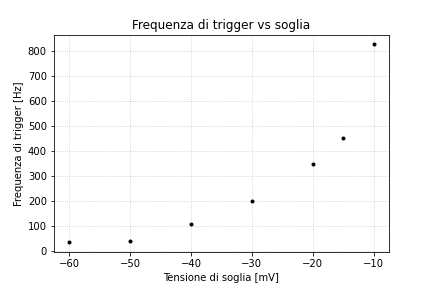
\includegraphics[scale=0.9]{ftrigger_vs_soglia.png}
\caption{Stima della frequenza di trigger media al variare della soglia di trigger} \label{f1}
\end{center}
\end{figure}

\subsection{Studio del segnale in uscita dal discriminatore}
Ho poi collegato il segnale in uscita da PM7 all'input di un canale del discriminatore ed ho visualizzato all'oscilloscopio sia il segnale di PM7 sia quello in uscita dal discriminatore. \\
Ho modificato le impostazioni del discriminatore, in modo da avere una soglia di -40 mV e un segnale della durata di circa 50 ns.\\
Con queste impostazioni, il segnale in uscita dal discriminatore è un segnale costante con il minimo a -1 V che si azzera di nuovo dopo circa 50 ns.
\paragraph{Stima del ritardo introdotto dal discriminatore} A partire dalle forme d'onda osservate sull'oscilloscopio ho stimato il ritardo introdotto dal discriminatore rispetto al segnale del fotomoltiplicatore.\\
Cavi usati per i collegamenti:
\begin{itemize}
    \item Collegamento PM7-input del discriminatore: cavo con ritardo di 2 ns
    \item Collegamento input del discriminatore - CH1 dell'oscilloscopio: cavo con ritardo di 2 ns
     \item Collegamento output del discriminatore - CH2 dell'oscilloscopio: cavo con ritardo di 4 ns
\end{itemize}
Con questi cavi il ritardo che si osserva sull'oscilloscopio tra il segnale del fotomoltiplicatore e quello del discriminatore è proprio il ritardo introdotto dal discriminatore. Infatti il segnale di PM7 impiega un tempo di 2ns+2ns = 4ns per arrivare sull'oscilloscopio attraverso i due cavi, mentre quello in uscita dal discriminatore 4ns attraverso il cavo più lungo.
\\
Ho misurato con i cursori dell'oscilloscopio i due tempi a cui il segnale del fotomoltiplicatore e del discriminatore sono a circa metà della loro discesa. In particolare, per un singolo segnale ho misurato le seguenti quantità: 

\begin{table}[h!]
    \centering
    \begin{tabular}{|c|c|c|}
        \hline
        Canale & Minimo del segnale & Istante di tempo a cui il segnale è a metà\\
        \hline
            CH1 & -79.2 mV & -2.00 ns \\
            CH2 & -1.06 V & 14.2 ns   \\
        \hline
    \end{tabular}
    \caption{Dati per la stima del ritardo introdotto dal discriminatore}
    \label{tab1}
\end{table}


Da questa misura si ricava che il ritardo introdotto dal solo discriminatore è di 16.2 ns. Se invece vogliamo considerare anche il ritardo introdotto dai cavi rispetto al momento in cui il segnale parte dal rack, bisogna aggiungere 4 ns.

\subsection{Contatore NIM in singola}
Ho collegato il segnale in uscita dal discriminatore a un ingresso del contatore NIM, in modo da contare il numero di eventi per unità di tempo e confrontare questo risultato con la frequenza di trigger dell'oscilloscopio. \\
\\Impostazioni del discriminatore e del contatore: 
\begin{itemize}
    \item Soglia del discriminatore: -40 mV
    \item Durata del conteggio: 10000 cicli di clock, cioè 10s
\end{itemize}
\paragraph{Terminazione del cavo che collega l'uscita del discriminatore all'ingresso del contatore}
Dato che la resistenza in ingresso del contatore è di 50 Ohm, si può collegare direttamente l'uscita del discriminatore all'ingresso del contatore senza terminare con una resistenza da 50 Ohm. Ho provato però ad aggiungere comunque una T con un tappo da 50 Ohm e i conteggi sono circa raddoppiati. Questo effetto è dovuto alle riflessioni del segnale nel cavo coassiale se non trova in uscita la stessa impedenza interna del cavo. 
\\
Ho notato però un fenomeno curioso: i conteggi raddoppiano se aggiungo un tappo da 50 Ohm raddoppiano solo in alcuni ingressi del contatore NIM, mentre in altri il numero di eventi per unità di tempo è circa lo stesso con e senza la resistenza aggiuntiva.
\\
In ogni caso, tutte le misure sono state prese senza aggiungere il tappo da 50 Ohm all'ingresso del contatore NIM.
\subsubsection{Confronto tra i conteggi e la frequenza di trigger} Idealmente, impostando la stessa soglia per il discriminatore e per il trigger dell'oscilloscopio, la frequenza di trigger e il numero di conteggi al secondo dovrebbero essere uguali, o almeno dello stesso ordine di grandezza. \\
Ho quindi provato ad impostare per entrambi una soglia di -40 mV ed ho misurato un numero di conteggi in 10 s pari a 1623. Quindi il numero di conteggi al secondo era 162.3 s$^{-1}$, ma la frequenza di trigger media era tra i 30 e i 40 Hz. \\
\\
Una possibile spiegazione di questa discordanza può essere il fatto che la soglia dell'oscilloscopio in realtà è diversa dai -40 mV. \\Ho infatti cambiato manualmente la soglia dell'oscilloscopio fino ad arrivare alla situazione in cui a volte il segnale del discriminatore era costantemente 0 mentre quello del fotomoltiplicatore era visualizzato all'oscilloscopio, ovvero fino a una tensione di soglia per il trigger di -21.6 mV. \\ Questa nuova soglia per il trigger perché è più alta della soglia effettiva che fa scattare il discriminatore: il segnale del discriminatore è nullo quando il segnale del fotomoltiplicatore è sotto la soglia di trigger ma sopra la soglia del discriminatore. \\Se però si sceglie la tensione di soglia per cui gli eventi in cui il discriminatore è nullo sono pochi, allora la soglia di trigger è abbastanza vicina a quella del discriminatore.\\
Infatti, con la soglia di trigger impostata a -21.6 mV la frequenza di trigger è in media 140-150 Hz, molto più vicina ai 162.3 conteggi al secondo misurati con il contatore.
\\
Ho quindi deciso di lasciare la soglia dell'oscilloscopio a -21.6 mV.
\subsubsection{Numero di conteggi per unità di tempo al variare della tensione di alimentazione del fotomoltiplicatore}

Ho poi cambiato la tensione di alimentazione del fotomoltiplicatore e ogni volta attivato il contatore per 10 s, in modo da vedere come cambia il numero di conteggi al secondo con la tensione di alimentazione. \\
In figura \ref{f2} ho riportato il grafico del numero di conteggi al secondo al variare della tensione di alimentazione in un range tra 1.60 e 1.975 kV. 
Da notare che la scala verticale è logaritimica, perché il numero di conteggi al secondo aumenta molto velocemente. L'andamento sembra quello di una legge di potenza.


\begin{figure}[h]
\begin{center}
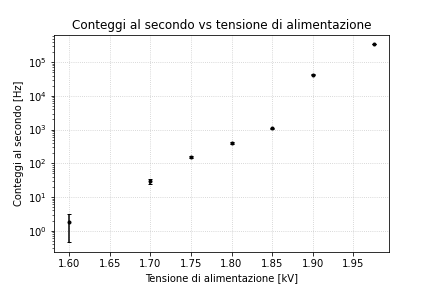
\includegraphics[scale=0.9]{conteggi_vs_alimentazione.png}
\caption{Andamento del numero di conteggi al secondo al variare della tensione di alimentazione del fotomoltiplicatore} \label{f2}
\end{center}
\end{figure}

\section{Studio dei tre fotomoltiplicatori più in alto (PM7, PM5 e PM4)}
Ho ripetuto alcune misure descritte nella parte precedente anche per i due fotomoltiplicatori posti sotto a PM7, ovvero PM5 e PM4. \\
In particolare, per prima cosa ho collegato i fotomoltiplicatori al discriminatore e al contatore, in modo da trovare la tensione di alimentazione per cui il numero di conteggi  per unità di tempo era intorno ai 100 cps.
\\
Come impostazioni sui due canali del discriminatore per PM5 e PM7 ho usato le stesse per PM7, ovvero tensione di soglia a -40 mV e durata del segnale discriminato di circa 50 ns. 
\\
Per avere un numero di conteggi per unità di tempo costante pari a circa 100 cps bisogna alimentare in modo diverso il fotomoltiplicatore nel mezzo (PM5) rispetto agli altri due. In tabella \ref{tab2} ho riportato le tensioni di alimentazione per cui si hanno circa 100 conteggi per secondo per ognuno dei tre fotomoltiplicatori. 
\\
\\
RIPRENDERE DATI
??PM7 e PM4 con alimentazione 1680 V, mentre PM5 con alimentazione 1580 V. 
In questo modo ho frequenze di circa 130 Hz su tutti e tre. ??
\begin{table}[h!]
    \centering
    \begin{tabular}{|c|c|c|}
        \hline
        Fotomoltiplicatore & Tensione di alimentazione [kV] & Conteggi per secondo\\
        \hline
            PM7 & 1.740 & !!!!   \\
            PM5 & ??? & !!!!   \\
            PM4 & ??? & !!!!   \\
        \hline
    \end{tabular}
    \caption{Tensioni di alimentazione e conteggi in singola per i tre fotomoltiplicatori}
    \label{tab2}
\end{table}

\section{Unità di coincidenza}
Nel rack sono presenti due unità di coincidenza, ognuna con cinque ingressi e due tipi di uscita, LIN e OUT. 
La prima è un segnale che è diverso da zero per l'intervallo temporale in cui tutti gli ingressi attivati sono contempoareamente accesi, mentre il secondo è un breve impulso di durata ????? che si attiva quando l'unità rileva una coincidenza tra i segnali in ingresso. 

\subsection{Ritardo introdotto dall'unità di coincidenza}
Per prima cosa, ho studiato le coincidenze tra i primi due fotomoltiplicatori (PM7 e PM5), collegando i rispettivi segnali discriminati a due ingressi di un'unità di coincidenza.\\
Ho visualizzato all'oscilloscopio i due segnali discriminati di PM7 e di PM5 e le due uscite dell'unità di coincidenza, LIN e OUT, in modo da stimare il ritardo introdotto dall'unità di coincidenza. 
\\
\\
Cavi usati per i collegamenti: 
\begin{itemize}
    \item Collegamento uscita discriminatori-ingresso coincidenza: cavi con ritardo di 2 ns
    \item Collegamento uscita discriminatori-oscilloscopio: cavi con ritardo di 2 ns
     \item Collegamento uscita LIN dell'unità di coincidenza-oscilloscopio: 4ns
\end{itemize}
In questo modo, il ritardo che si osserva all'oscilloscopio tra i segnali discriminati e il segnale in uscita dall'unità di coincidenza è proprio quello introdotto da quest'ultima. 
\\
\\
Ho quindi misurato con i cursori dell'oscilloscopio gli istanti di tempo in cui i segnali discriminati dei due fotomoltiplicatori (visualizzati in CH1 e CH2) e il segnale in uscita dall'unità di coincidenza (visualizzato in CH) sono scesi a metà della loro ampiezza, ottenendo i seguenti risultati: 

\begin{table}[h!]
    \centering
    \begin{tabular}{|c|c|c|}
        \hline
        Canale & Minimo del segnale & Istante di tempo a cui il segnale è a metà\\
        \hline
            CH1 (PM7 discriminato) & -992 mV & 6 ns \\
            CH2 (PM5 discriminato)& --912 mV& 0.7 ns   \\
            CH4 (uscita LIN unità di coincidenza) & -8.40 V & 15 ns\\
        \hline
    \end{tabular}
    \caption{Dati per la stima del ritardo introdotto dall'unità di coincidenza}
    \label{tab3}
\end{table}
A partire da queste misure ho stimato il ritardo introdotto dall'unità di coincidenza come la differenza tra il tempo in cui è scattato il primo fotomoltiplicatore (6 ns) e il tempo in cui è scattata l'unità di coincidenza, ottenendo un ritardo di 9 ns.

\subsection{Conteggi delle coincidenze doppie}



\end{document}